\chapter{Implementation Details}


From the previous section we saw that neglecting colour gradient affects shear measurements . Main target of our simulation is
to create a relaistic lensing effect. Galaxies were specified by different parameters and a particular distance from lens. We chose
comparitively simple model ''singular isothermal sphere'' for lens in the simulation. Initially we considered only monochromatic simulation,
i.e. our simulation ran only once for one wavelength and convolution was done using one PSF. Then we modified our programme so that instead
of running for one wavelength the simulation now runs for multiple wavelength range. We
took the infrared wavelength range 1.57$\mu m $-2.00$\mu m $ and didvided this range into 20 parts.  During this step galaxies were taken which have different
flux on two different bands ''f606w''(blue)  and ''f818''(red).In our simulations we mentioned them as ''blue'' and ''red'' galaxies.Linear
interpolation according to specific wavelength was done by using these galaxies to create galaxy samples which have
a certain percent of red and certain percent of blue flux. These galaxies were then convolved with the PSF of that particular range. We ran
the simulation for $90^{\circ}$ rotated angle also so that when combined the two output the net intrinsic ellipticity of the galaxy
shape can be avoided.

Our aim is to see how the psf affects shear measurements. To do so,I used the programme ``jedisim'' written by Dell Antonio.In this programme we run
a python script  named ``jedimaster.py'' . This script reads from a text file named ``config'' . This text file contains the information about different parameters.
``jedimaster.py'' runs six C programmes which creates the simulation step by step
The steps are given below

\paragraph{Postage stamps}:

 The images were obtained from an HST UDF image. From that image individual galaxies are converted into 600 by 600 pixel postage stamps.
In the postage stamps the galaxy is isolated on a blank background. The resolution of the images are 0.03 arc second per pixel.We took total 128 postage stamps so that our sample contains diverse
set of galaxy shapes and orientations.


\paragraph{Making the catalog}

  The c programme ``jedicatalog.c'' creates a realistic galaxy catalog.This catalog contains the information of galaxy images to be created. There were some parameters which were specified for each galaxy to be created. These paarameters are
discussed below

1.Magnitude

  We choose the magnitude of each galaxy to be in the range 22$\leq$M$\leq$28
The distribution is given by Power law
\begin{equation}
 P(M+dM)\propto 10^{BM}
 \end{equation}
 where M is the magnitude and B is the constant $ B = 0.33 $
We take zero point magniyude to be M=30

2.Radius

  HdF catalogs contains database of r50 galaxies. That database was binned by integer part of the magnitude
and a list of  radii is made for each magnitude bin.As we have already assigned a magnitude for our galaxy this magnitude
corresponds to a particular bin and a r50 radius was randomly chosen from that bin

3.Redshift

 In general different galaxies have different redshift but for our simulation we take all the galaxies to be at
a single redshift. All the background galaxies are in redshift $ z = 1.5 $ and lens is at $ z= 0.3 $

4.Position

 The center of the postage stamps were selected from the range [301,40960] so that the whole gakaxy fits within image and edge effect can e avoided

5.Angle

 As the universe is homogenous and isotropic galaxies are in general randomly oriented in the sky. The 'jedicatalog.c' programme randomly
choose an angle from the range[0,2$\pi$]. In general the orientation has 3 degress of freedom but as we are dealing with 2D projection of galaxies,we can make the orientation random in only 1 degress of freedom

So in general 'Jedicatalog.c' creates a catalog which contains the name of source postage stamps,the radius,magnitude,redshift,angle and the galaxy image name which to be created in the next step.

\paragraph{Transforming the galaxy according to the catalog}:

'Jeditransfom.c' takes the catalog and source postage stamps. The postage stamps are then scaled down to corrected radius, the flux is adjusted for image according to
the magnitude which was specified in the catalog and each galaxy is rotated through the assinged angle.The postage stamps are then cut out so that
the final image contains all the non zero pixel of the galaxy
From Figure 2.1 we see a sample postage stamp and the same stamp(lower figure) transformed according to parameter

\begin{figure}[ht]
\begin{center}
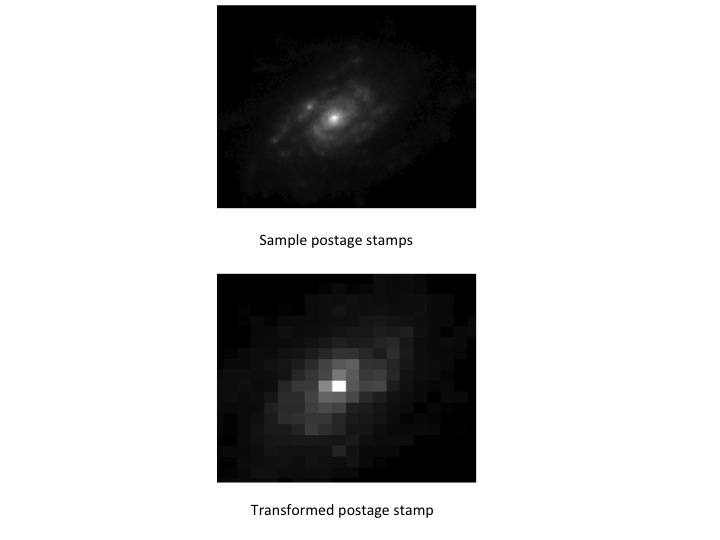
\includegraphics[width=15cm,height=15cm]{pos.jpg}
\label{fig}
\caption{Postage Stamp transformed according to the parameters in catalog}
\end{center}
\end{figure}

\clearpage

\paragraph{Distorting the galaxies}

As we have seen before in the weak field limit for a point mass, the lens equation is

\begin{equation}
\begin{split}
 \vec\beta(\vec\theta) &= \vec\theta - \vec\alpha(\theta) \\
                       &= \theta - \frac{D_{ls}}{D_s}  \vec\hat\alpha(\vec\theta)
\end{split}
\end{equation}

We consider here the lens as a symmetric mass distribution with the center at arbitrary positionand redshift at z=0.3 . the deflection term in the lens equation becomes

\begin{equation}
 \vec\hat\alpha(\vec\theta) = \alpha(r) {\vec\hat r}
\end{equation}

where $\alpha(r)$ is the radial deflection which depends upon mass distribution.

There are two types of mass distribution :

1. Singular Isothermal Sphere:

2. Navarro Frenk White Profile

We are considering only Singular Isothermal Sphere(SIS) profile. For this profile the density is given by

\begin{equation}
 \rho = \frac{\sigma^2_v}{2 \pi Gr^2}
\end{equation}

Here $\sigma_v$ is velocity dispersion, G is universal gravitational constant. When r$\rightarrow$ 0 the density $\rho \rightarrow \infty $.
So we see that at r=0 this is not a physical situation. But as long as it is finitely bounded it constitutes a possible physical distribution and can be used as lens.

The deflection in pixels due to an SIS profile is given by

\begin{equation}
 \frac{\alpha(r, \sigma_v) }{r} = \frac{4\pi}{r} (\frac{\sigma_v}{c})^2 S
\end{equation}

Where S is the conversion factor between pixels and radians given by

\begin{equation}
S = \frac{\pi}{180} \frac{3600}{resolution}
\end{equation}

So We have seen that the amount of distortion depends upon the deistance between the lens and galaxy. The lens position was selected
to be (6144,6144).

If we take a galaxy at position(5754,7909) then the distance from the lens to the galaxy is

\begin{equation}
\begin{split}
 r_1 &= \sqrt{(6144-5744)^2 + (6144-7909)^2} \\
     &= 1809.75
 \end{split}
\end{equation}


Similarly if we take another galaxy which is at position(690,5217) the distance from the lens for this second galaxy would be

\begin{equation}
\begin{split}
 r_1 &= \sqrt{(6144-690)^2 + (6144-5217)^2} \\
     &= 5532.21
 \end{split}
\end{equation}

From equation (50) we see that deflection is inversely propotional to r i.e the galaxies are at larger position from lens
would be deflected less than the galaxies at nearby position. So according to the value of $ r_1 $ and $ r_2$ galaxy 1 would be distorted more than galaxy 2


\paragraph{Embedding all the unconvolved image}

 'Jedidistort.c' simulated the distortion effect in all the galaxies. It also specified two keywords 'xembed' and 'yembed' in the
fits image . 'xembed' and 'yembed' means x and y cordinate of lower left pixel if the individual image is to be embedded on a larger
image . 'Jedipaste' takes all these 12000 images and embedds them on to a larger image which is 12288 by 12288 pixel.
Due to computer memory allocation problem ''jedipaste.c'' can't embedds all these large number of images into a single huge image
at once.Instead it divides the larger image(12288,12288) into two equal rectangular parts which was called 'bands' in our programme.
So band1 has cordinates where x range is (0,12288) and y range is (0,6144) . band 2 has xrange smae as band 1 but y range is from(6144,1288).
''jedipaste.c'' then takes all these image and embedds images according to their 'xembedd' and 'yembed' co-ordinate position in
first in band 0 and then in band 1.


\paragraph{Convolution with PSF}

The light from the distant galaxies not only gets deflected by the intervening gravitational field of the forground sources but also
gets affected by the Telescope Optics.This effect is known as PSF which we discussed above(Section 1.4)

In general we can write convolution of two functions f(x) and g(x) as


\begin{equation}
 f(x)*g(x) = \int f(y)g(x-y)dy
\end{equation}

If there are n data points then from the above equation we see that we need to calculate $ n^2$ tems for each times
For am image with size 12288 pixel by 12288 pixel this is not so practicle. That's why in this case we take Fourier transform of the image and psf and use convolution theorem.
The convolution theorem states that

\begin{equation}
F(f*g) = F(f(x))\bigotimes F(g(x))
\end{equation}


The programme 'Jediconvolve.c' uses the 'fftw3' library to implement this idea. This is a very fast procedure to obtain the convolved image.

In the programme 'jediconvolve.c' it reads the pixels of the image by using the array pImg and pixels of Psf using the array pPsf.
Under the 'fftw3' there are some plans for example we used fftw\_plan\_dft\_r2c\_2d. When these plans are executed we get the Fourier transform of the object.For example
we used fftwf\_execute(pPIMg). takes the fourier transform of the image array. Similarly it also does the same procedure for 'PSF' array.

The image after the convolution is still in the frequency sapce,so the inverse transform was taken to get it in real space.

As the image 'HST0.fits' is very large(12288 by 12288 pixel) the programme cant take it at once. so the programme divides the whole image into 6 bands. so in each band there are 2048 pixels.
Each of this band was Fourier transformed and then convolved with the fourier transform of the PSF and the output of this image was taken reverse fourier transform.
As there are total 6 bands we get 6 images


\paragraph{Making Convolved Image}

The''jediconvolve.c'' creates 6 images. The jedipaste programme once again takes this 6 images and reads the x and y co ordinate of the lower left pixel.
It then divides the whole image into  2 rectangular parts 'band 0' and 'band 1' and embedds these images respectively in those two bands and creates one final image ``HST\_convolved.fits''


From figure 2.2  we can get an idea how the galaxies are embedded in large file


\begin{figure}[ht]
\begin{center}
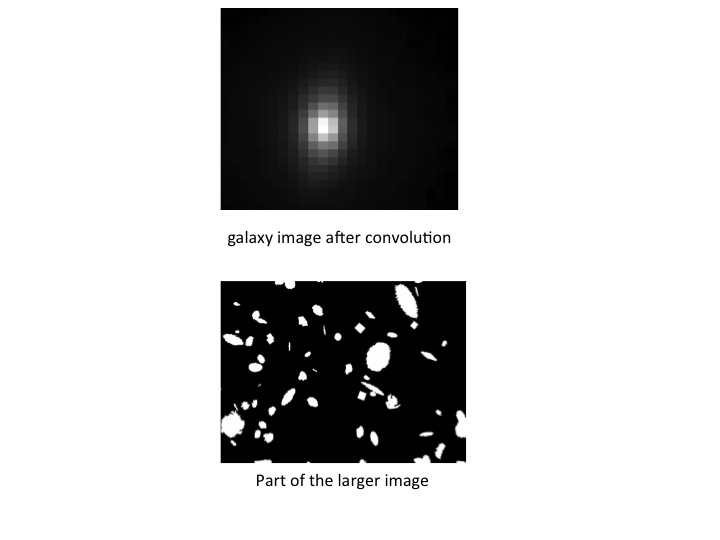
\includegraphics[width=15cm,height=15cm]{con.jpg}
\label{fig}
\caption{Convolved and distorted galaxy image}
\end{center}
\end{figure}


\paragraph{Rescaling accroding to the resolution of WFIRST}

The resolution of the image ``Jedipaste.c''  creates is 0.03 arcsecond.But the WFIRST has resolution 0.11 arcsecond. So ``jedirescale.c'' mainly scales
down this image into a larger pixelscale and trims off the border.It finds the box which each pixel makes on the image,integrates over the area
under that box,averages  and assings that value to new pixel.

\paragraph{Adding Noise to the image}


 Finally there are some random noise associated with each image. 'Jedinoise.c' added the poisson noise of mean value 10 to the final
image ``LSST\_convolved\_noise.fits''. WE tried to keep noise as low as possible in our simulation so that it does not effect in shear measurement.

\paragraph{Changes Made to original programme}

\paragraph{Implementing wavelength dependence}
   Preliminary we worked only on monochromatic images. We obtained 100 images in ``f608'' filter and another 100 images in ``f814'' filter.These
images are also 0.03 arcsecond per pixel as before.

  To test the color dependency we took wavelength at 1.57-2.00 range.Then we divided this range into 20 parts
 I edited the Jedisim programme in a way so that unlike the first part instead of running for only one time now it runs for 21 times.

  I  wrote one programme 'color.c' which would take this blue and red images and creates the final image by linear interpolation


In terms of equation for any run n

\begin{equation}
  output image = (1-\frac{n}{20})* blue image + \frac{n}{20}*red image
\end{equation}

We wrote the formula because the wavelength is going from blue to red. So when $n=0$ i.e. the wavelength is 1.57 the blue image would contribute most and when $n=21$
(wavelength 2.00)the red images would be dominant

Previously during the convolution the Psf was monochromatic. But now we need the PSF which would depend upon the wavelenth. We got 21 wavelength dependent PSf from the website.
$http://localhost:8888/notebooks/WebbPSF\-WFIRST\_Tutorial.ipynb$

The PSF's are wavelength dependent so as the wavelength increases the FWHM also increases
It follows the same step as before but instead of one output after ``jedirescale.c''  the programme produces 21 output. I wrote one programme
``avg20.c'' which takes this 21 output. It averages them and create one image ``LSST\_convolved.fits''. In the final step the noise was added using the programme ``Jedinoise.c'' as before


Similarly the programme also runs for the 90 rotated case as before



\chapter{Results}



\subsection{Weighted Average of PSF}

One of the main purpose of the study is to observe how PSF size changes lineraly or follows any particular form as
a function of wavelength.PSFs are in general estimated using stellar spectra. For a given wavelength range different stars
have different spectral energy distribution.Finding flux for a particular PSF in that range enbles us to find flux weighted
average of the PSF. This in turn helps us to compare the size of PSF for different wavelength regions

I downloaded 15 stellar SED text file from the website $http:$//irtfweb.ifa.hawaii.edu$/~spex/IRTF\_Spectral\_Library/$. The SED's were taken for
F,G,M,K,L stars .

I wrote a programme ''readf2.py'' to find flux for each 21 psf files. This programmes reads from the Spectral energy distrinution(SED)
file.For example we need flux at particular value $ x_i$  . So the programme finds from SED file two nearby values $ x_{i-1}$ and $ x_{i+1}$ and the
corresponding flux value $ y_{i-1}$ and $ y_{i+1}$ . Then it linearly interpolates between those two points

So the slope m is

\begin{equation}
 m = \frac{y_{i+1}-y_{i-1}}{x_{i+1}-x_{i-1}}
\end{equation}

Once we got the slope ,the y intercept for that straight line is

\begin{equation}
 c = y_{i+1} - mx_{i+1}
\end{equation}

So if we now  subsitute the m and c in the straight line for a particular wavelength x the flux would be

\begin{equation}
 y = mx +c
\end{equation}

So this programme finds flux for each 21 wavelength and writes them to a text file.

We can see from  left side of Figure 3.1 when the flux from SED file and the interpolated fluxes are plotted vs wavelength

So the interpolated flux does not agree with the flux from SED. This is due to the fact that we took only nearby two points.Whereas
the SED varies a lot between two wavelength regions

So I wrote another programme ''newprac.py'' which takes the midpoint of each regions. For a particular value it integrates the flux
between those two midpoint values. For example if we need to know the flux at 1.5915(for psf1.fits file) the programme first find the value
at 1.58075 and 1.60225 by linear interpolation. Then it takes all the values between these points from SED files and integrate
over this range.

After making these changes the flux for SED file and psf files were plotted which we can see from right side of
Figure 3.1


I then wrote one programme ''pyfits2.py'' which finds the weighted average for the 21 PSF files.
For example for a star if $f(x_i) $ denotes the data value of the fits file and $x_i $ denotes the corresponding flux then the
weighted average would be

\begin{equation}
  \bar x = \frac{\sum_{n=1}^{21} f(x_i)x_i}{\sum_{n=1}^{21} x_i}
\end{equation}

\begin{figure}[ht]
\begin{center}
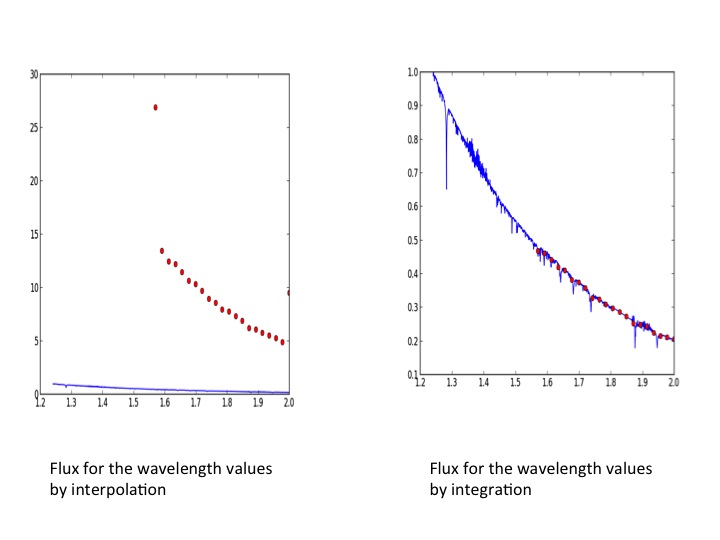
\includegraphics[width=15cm,height=15cm]{flux.jpg}
\label{fig}
\caption{Integrating flux from SED files for  wavelength}
\end{center}
\end{figure}


\clearpage

One of the main prupose is to study how the Psf cahnges with wavelength

To test this I wrote one programme ''inte.py''. this programme finds the flux ratio for two wavelength range one from (1.24-1.57) and
the other one is 1.57-2.00. Based upon the SED files it integrates over the wavlength ranges. Then it finds the absolutte magnitude which
was defined as a variable ''color'' in the programme

the magnitude is given byar

\begin{equation}
 m = -2.5 log(\frac{f_1}{f_2})
\end{equation}

where $f_1$ is the flux for first wavelength range and $f_2$ is for the second wavelength range.
